\graphicspath{{./figures}}

\section{Ground Station Antenna}

The ground station antenna's return loss was measured using a network analyser to ensure it was correctly matched to 50 ohm. The resultant graph is shown in Figure \ref{fig:helicalReturnLoss}. The figure shows the simple matching strip design is effective and was implemented correctly, however it should be noted that the null is not as deep as simulated (only around -10 dB minimum around 427 MHz as opposed to the -50 dB simulated results at the centre frequency of 433 MHz).

\begin{figure}[!htb]
  \centering
  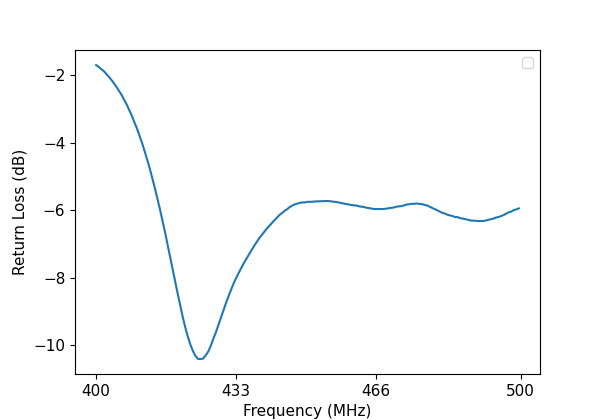
\includegraphics[width=0.8\textwidth]{helicalReturnLoss}
  \caption{Helical Antenna Return Loss vs Frequency}
  \label{fig:helicalReturnLoss}
\end{figure}

There are several reasons why the null may not be as deep as simulated. Firstly, the aluminium foil used is far from an ideal PEC. Secondly, the imperfections in the antenna's construction (e.g. bends in the wire, the PVC and wooden dielectrics that were not simulated, etc.) may cause the match to be non-ideal. Finally, although a short length matching strip performed well in simulations, it is hypothesized that a longer strip might have made the implementation more achieveable due to increased capacitive coupling. Instead of optimizing the antenna build, however, it was decided to run further tests with this system, since the link budget allows for up to a 1 dB matching loss. Optimization is therefore left for future projects. Lastly, the antenna gain pattern unfortunately could not be measured, as a chamber was not available that catered for the low frequency of the system.